\documentclass[12pt]{article}
%\usepackage[backend=biber]{biblatex}
\usepackage{amsmath}
\usepackage{listings}
\usepackage{graphicx}
\usepackage{caption}
\usepackage{subcaption}
\usepackage{commath}
\usepackage{hyperref}
\usepackage{url}
\usepackage{xcolor}
\usepackage{textcomp}
\usepackage{dirtytalk}
\usepackage{listings}
\usepackage{wasysym}
\usepackage{float}
\usepackage{listings}
\usepackage[linesnumbered,lined,boxed,commentsnumbered]{algorithm2e}

% Packages from derivations_fullproblem.tex
\usepackage[squaren]{SIunits}
\usepackage{a4wide}
\usepackage{array}
\usepackage{cancel}
\usepackage{amsmath}
\usepackage{amsfonts}
\usepackage{amssymb}
\usepackage{graphicx}
\usepackage{enumerate}

% Parameters for displaying code.
\lstset{language=C++}
\lstset{basicstyle=\ttfamily\small}
\lstset{frame=single}
\lstset{keywordstyle=\color{red}\bfseries}
\lstset{commentstyle=\itshape\color{blue}}
\lstset{showspaces=false}
\lstset{showstringspaces=false}
\lstset{showtabs=false}
\lstset{breaklines}

% Define new commands
\newcommand{\expect}[1]{\langle #1 \rangle}

% Add bibliography
\begin{document}


\title{MAT4110 - Oblig 1}
\author{Geir Tore Ulvik - ulvik}
\maketitle

\section{Linear Least Squares with QR- and Cholesky Factorization}
\begin{figure}
	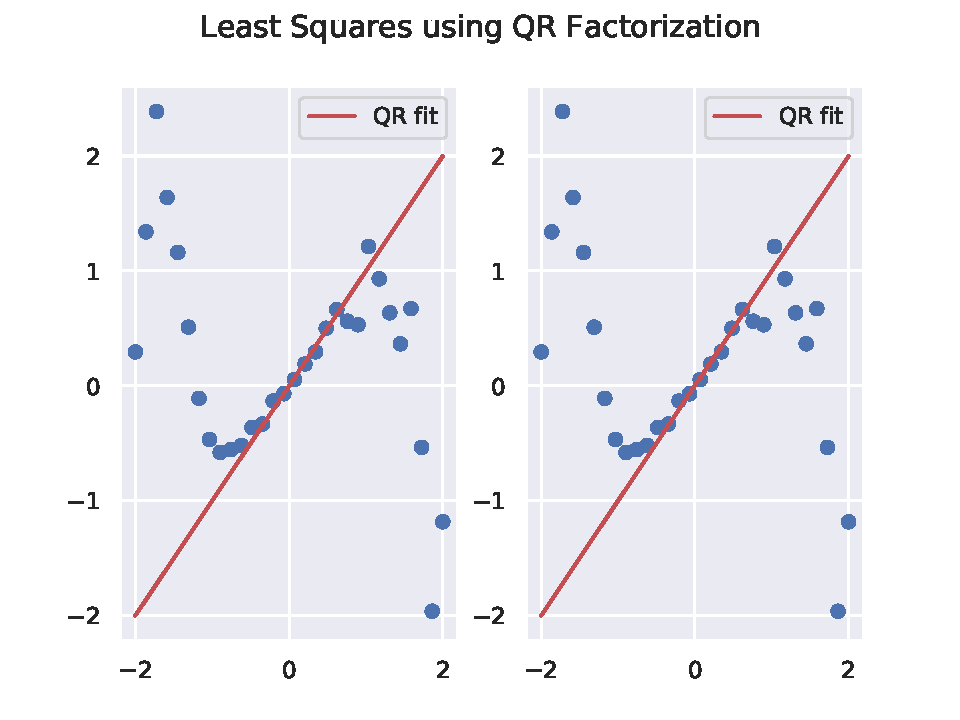
\includegraphics[width = \textwidth]{figures/QR.pdf}
	\caption{Plotted results of performing linear regression to solve the least squares
		problem using QR Factorization.}
\end{figure}
\begin{figure}
	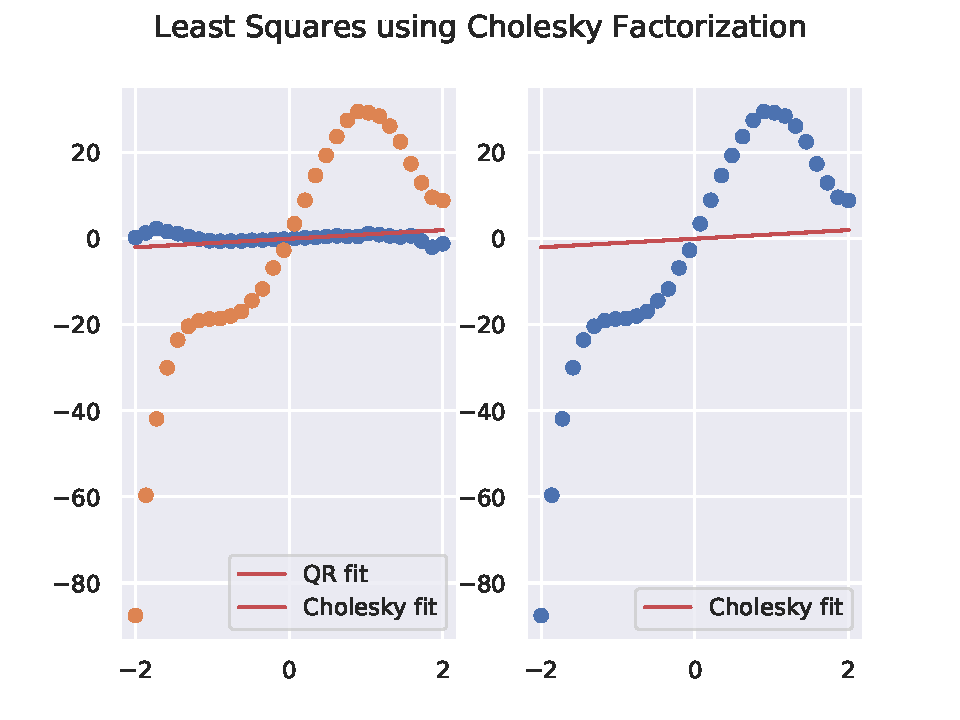
\includegraphics[width = \textwidth]{figures/Cholesky.pdf}
	\caption{Plotted results of performing linear regression to solve the least squares
		problem using Cholesky Factorization.}
\end{figure}


\end{document}
